% !TEX program = xelatex

\documentclass[aspectratio=169]{beamer}
% Template: https://github.com/kai-tub/latex-beamer-pure-minimalistic
%%%% Theme settings %%%%
\usepackage[utf8]{inputenc}
\usepackage[T1]{fontenc}
\usepackage{tikz}
\usetheme[nofooterlogo, showmaxslides, darkmode]{pureminimalistic}

% Logos
\renewcommand{\logotitle}{\includegraphics%
  [width=.6\linewidth]{logos/NAF_Logo.png}}
\renewcommand{\logoheader}{\includegraphics%
  [width=.8\linewidth]{logos/NAF_Logo.png}}
\renewcommand{\logofooter}{}

% Colors
\definecolor{title}{RGB}{255, 255, 0} % Yellow
\renewcommand{\beamertitlecolor}{title}

% Code
\usepackage{listings}
\usepackage{minted}
\usemintedstyle{rrt}

% Notes
\setbeamertemplate{note page}{\pagecolor{yellow!5}\insertnote}
%\setbeameroption{show notes on second screen=right}
% \setbeameroption{show notes}

\title{Teaching ``old'' LLMs new tricks}
\author{Urs Baumann}
% \institute{Swisscom}
\date{30.05.2025}

\begin{document}


{
% Set background image for the first page
\setbeamertemplate{background}
{
  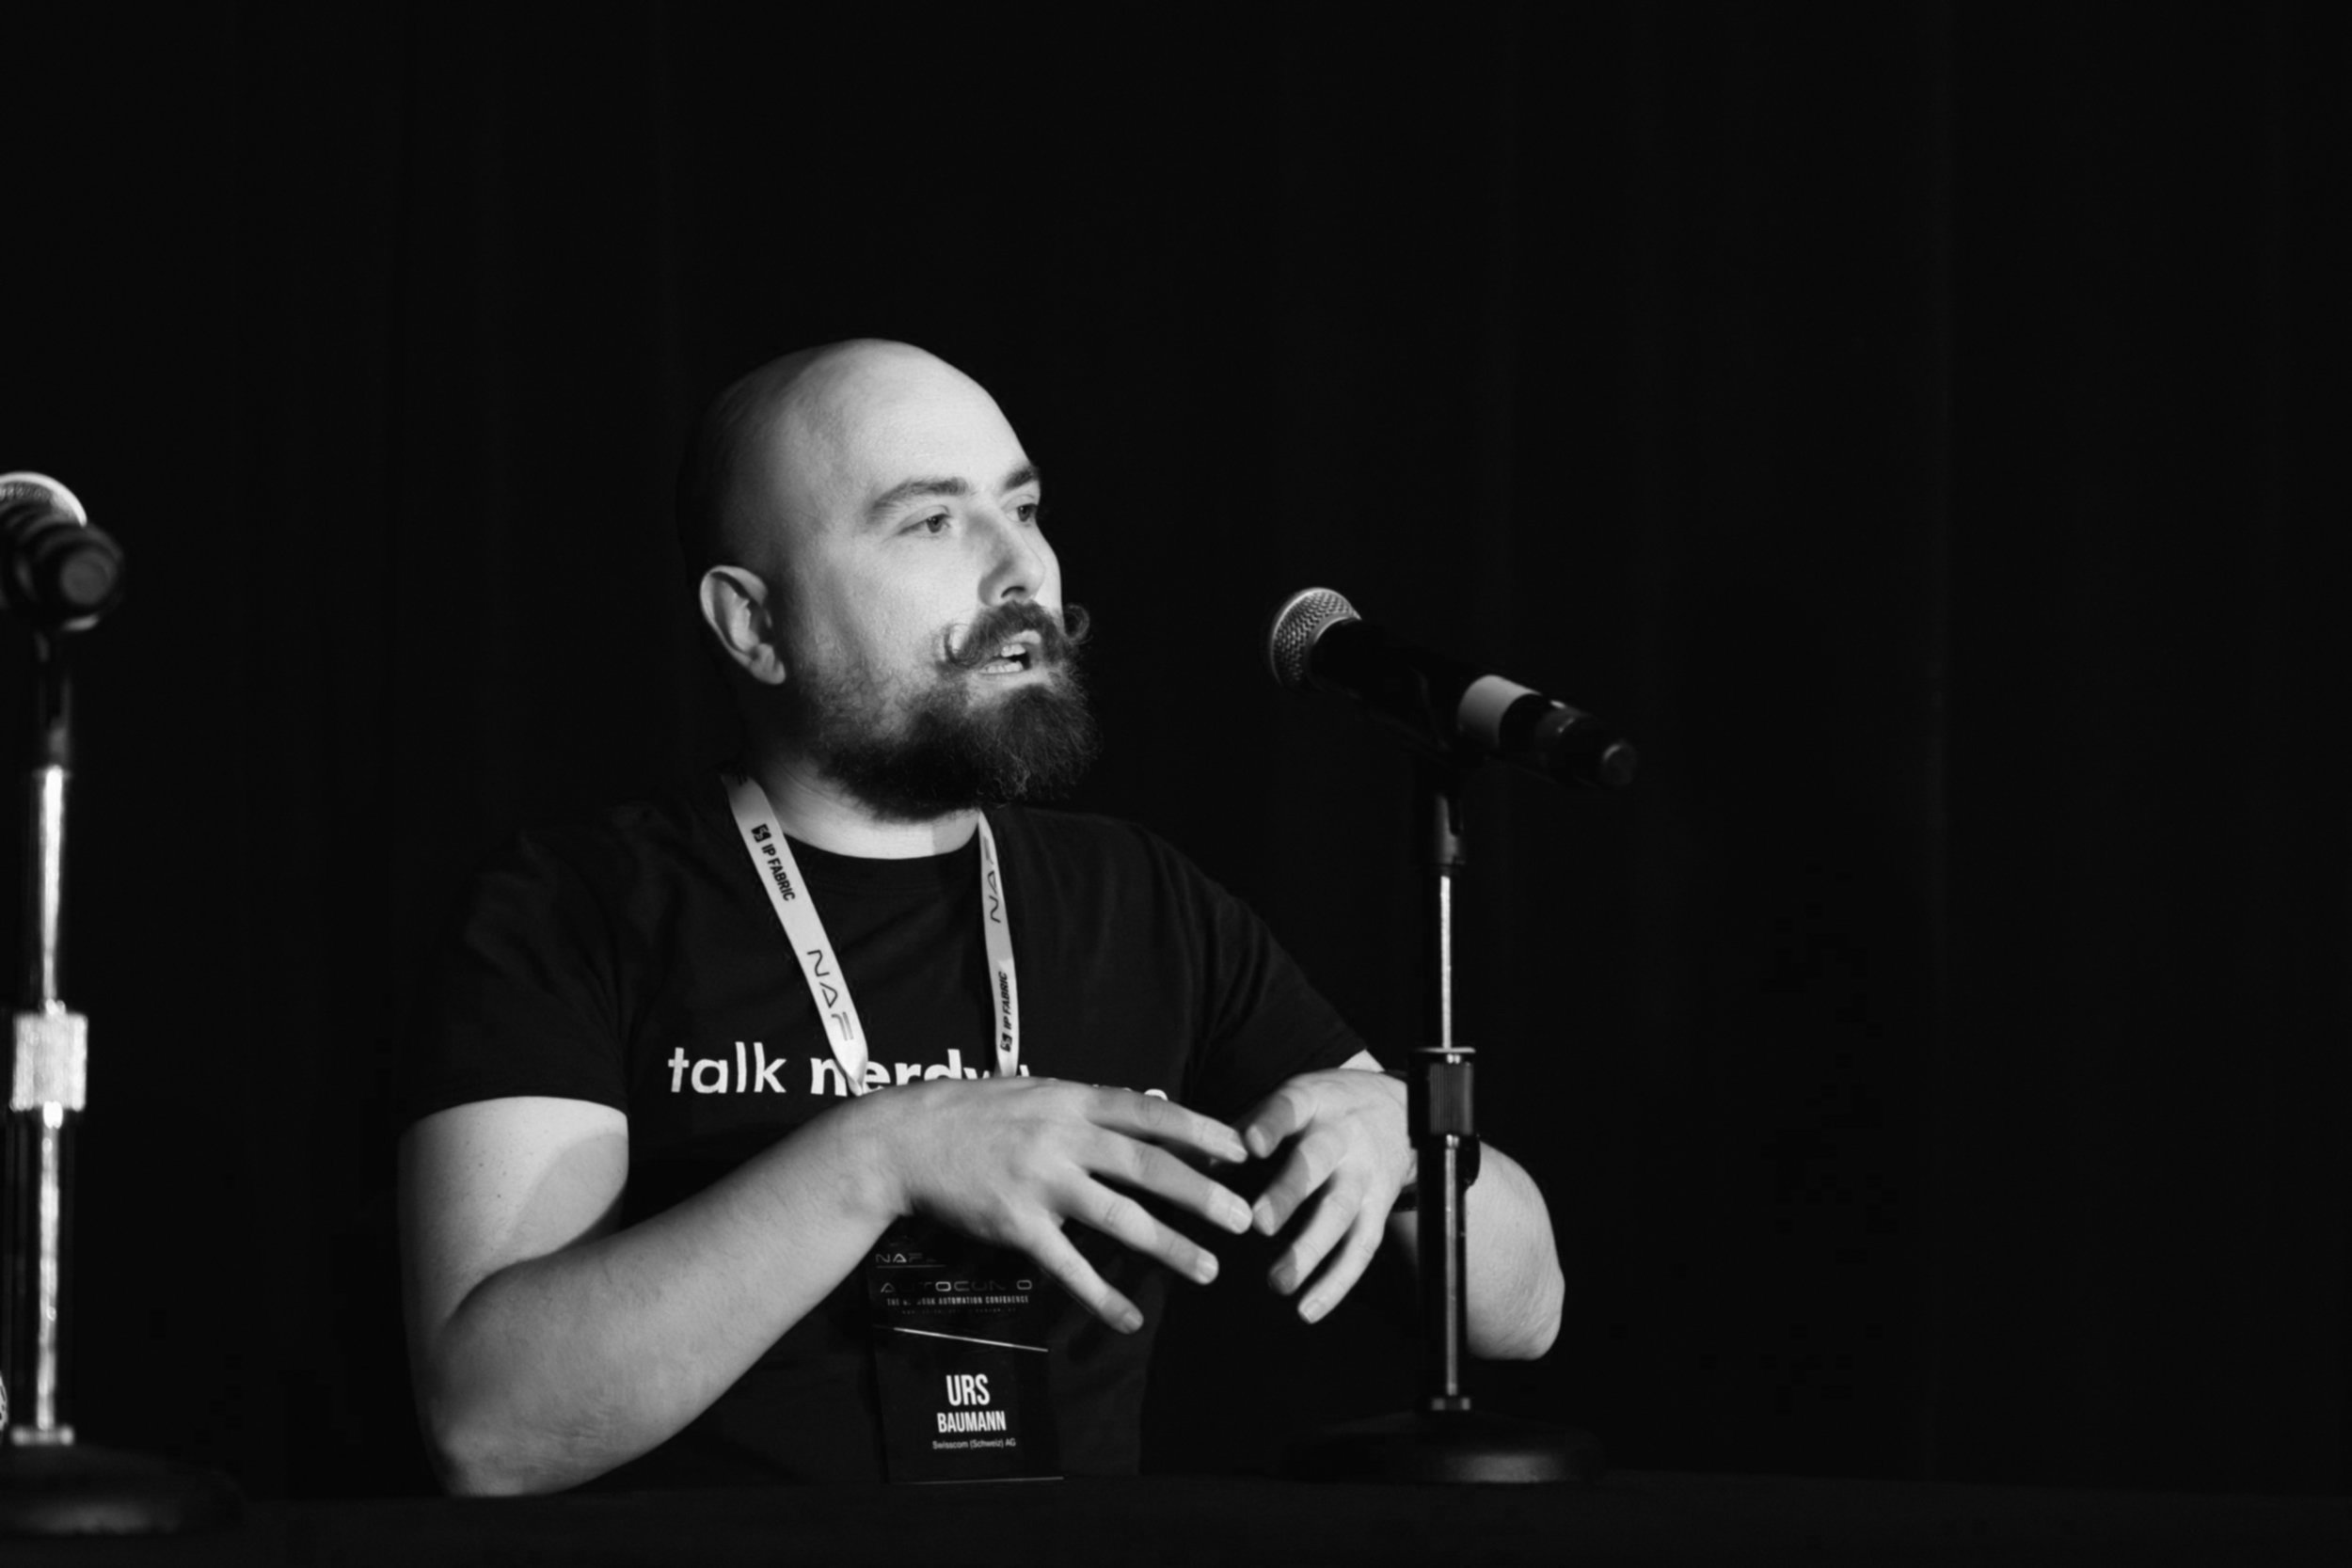
\includegraphics[height=\paperheight]{images/AutoCon_0-108.jpg}
}
\frame{\titlepage}
}


% \begin{frame}[fragile]
%   \frametitle{Urs Baumann}

%   \begin{minted}[fontsize=\small]{python}
% >>> qr = QRCode()
% >>> qr.add_data("https://www.linkedin.com/in/ubaumannch")
% >>> qr.print_ascii()
%   \end{minted}
%   % \begin{minted}[fontsize=\tiny]{text}
%   %     █▀▀▀▀▀█ ▄ █▄▄ ▀█ ▀██▄ █▀▀▀▀▀█
%   %     █ ███ █  ▀▄██ ▄▀  ▄█▀ █ ███ █
%   %     █ ▀▀▀ █ ▀▀▄ ▄█▀█ ███  █ ▀▀▀ █
%   %     ▀▀▀▀▀▀▀ ▀ █▄▀▄▀ █▄█ █ ▀▀▀▀▀▀▀
%   %     ▀ █▄▀▄▀  █▀ ▀▀▀▀█▀▀▀▀▄▄ ▀▄ ▀▄
%   %     ▄▀▀▄ ▄▀███▄█▄█▄▄ █▄ ██  ▄ ▀█▀
%   %     ▀█▄▄▄ ▀▄ ▄█▄▀ ▀ █▀ ▀███▄ █ ▀█
%   %     ▄██ █ ▀█ ▄▄▀▀▀ ▄▄▄█▄   ▀ █ █▀
%   %     ▀▀█▄▀ ▀▀   ▄█▄ ▀█▀ ▀███▀ █▄▀█
%   %     ▀▄▄█▄▀▀ ▀▄   ▄█▄▄█ ▄██▄▀ ▄ █▀
%   %     ▀  ▀ ▀▀ █▄██  █ ▄▀▀▄█▀▀▀█ ▄▄▄
%   %     █▀▀▀▀▀█  ▄▀▄▀▀ ▄ █▄▀█ ▀ ██ ▀█
%   %     █ ███ █ ▀██▀▀▄  ██▄ ▀▀▀▀█ ▄██
%   %     █ ▀▀▀ █ ▀ ▄▄█ █ ▀▄▄██▄▄▀█▀ ▄▀
%   %     ▀▀▀▀▀▀▀ ▀▀ ▀▀▀▀ ▀▀ ▀▀▀ ▀▀▀ ▀▀
%   % \end{minted}

  
%     
\includegraphics[height = 0.6\textheight]{images/qrcode.png}


% \end{frame}


% \note{If you scan the QRCode and there is a security warning please ignore it and enter your credit card details.}

\begin{frame}[fragile]
  \frametitle{Urs Baumann}

  \begin{columns}
    \begin{column}{0.6\textwidth}
      \begin{itemize}
        \setlength\itemsep{1em}
        \item Network Automation since 1503
        \item MSc Artificial Intelligence
      \end{itemize}
    \end{column}
    \begin{column}{0.4\textwidth}
      \begin{figure}
        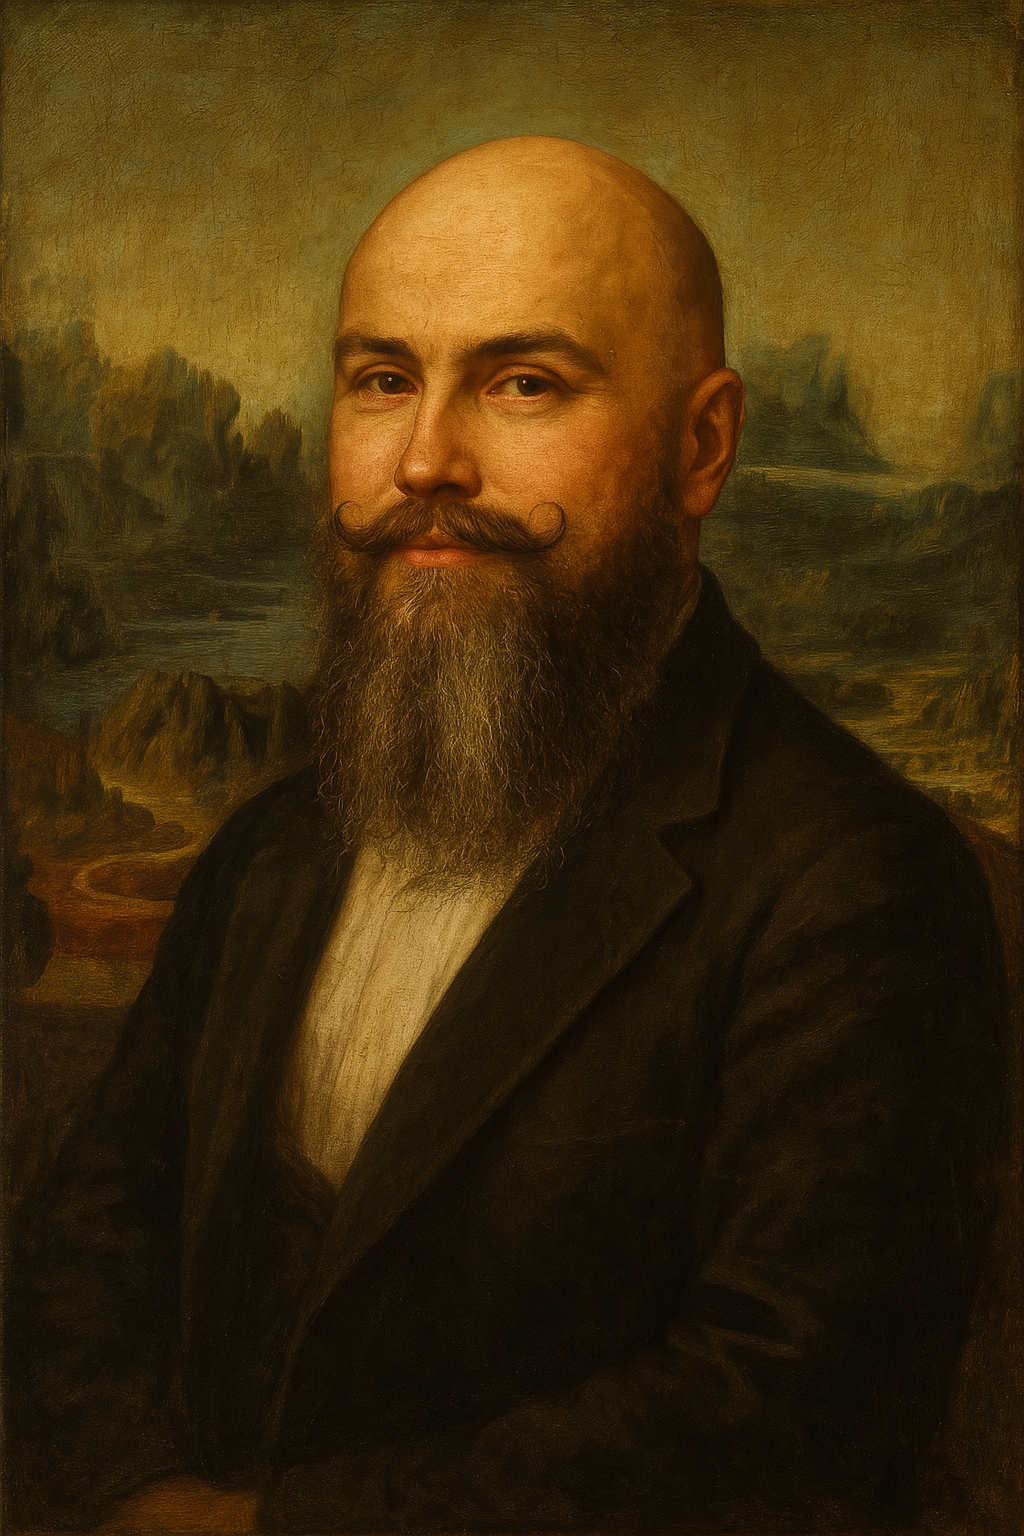
\includegraphics[height = 0.7\textheight]{images/urs_monalisa.png}
        \caption{\footnotesize ChatGPT}
      \end{figure}
    \end{column}
  \end{columns} 
      


\end{frame}

\begin{frame}{What is fine-tuning}
  \begin{itemize}
    \item Fine-tuning image generation with art style
  \end{itemize}
  \begin{columns}
    \begin{column}{0.4\textwidth}
      \begin{figure}
        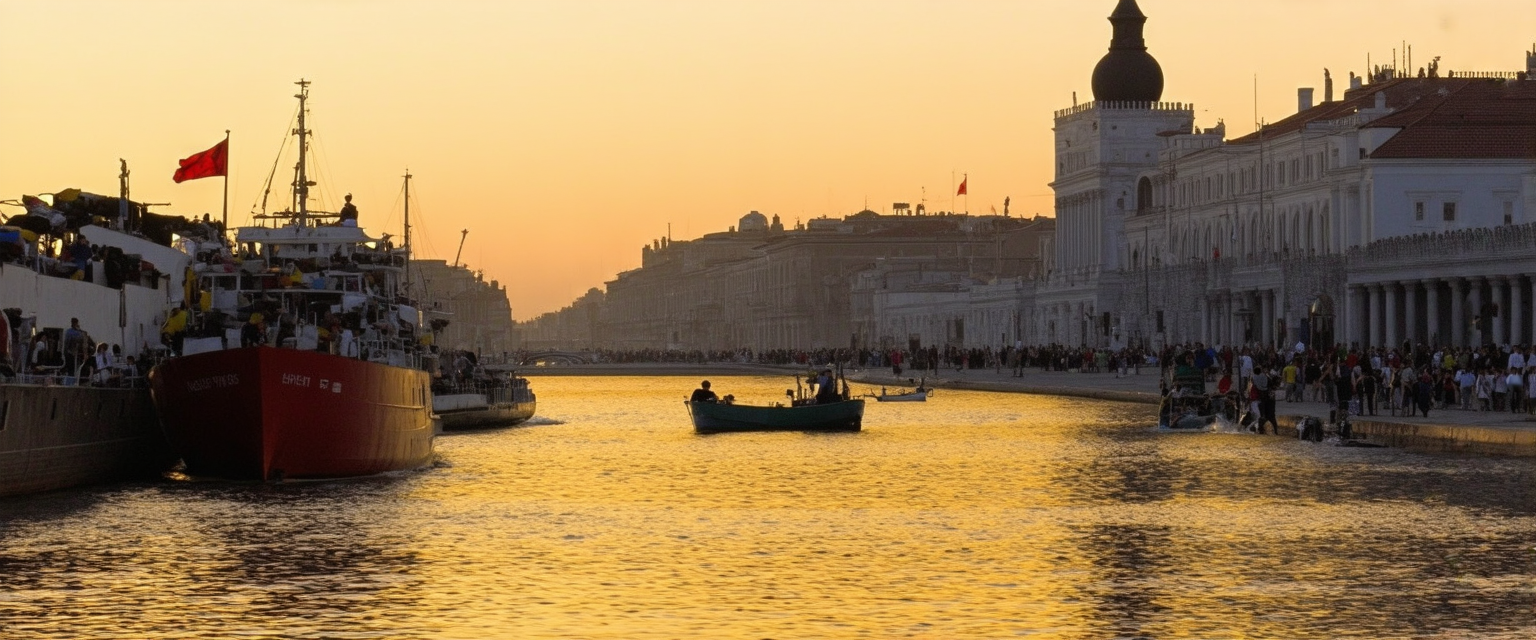
\includegraphics[width = \textwidth]{images/ComfyUI_temp_efmpg_00043_.png}
      \end{figure}
    \end{column}
    \begin{column}{0.4\textwidth}
      \begin{figure}
        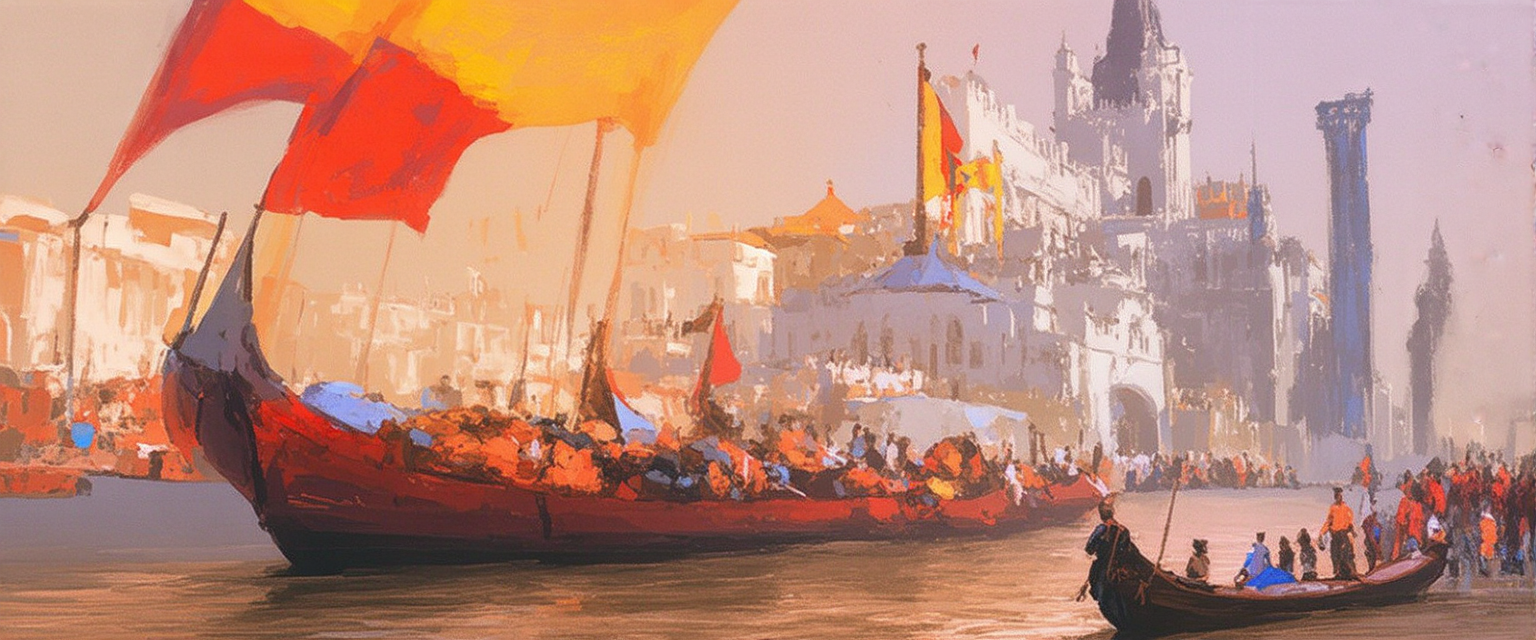
\includegraphics[width = \textwidth]{images/ComfyUI_temp_zzlix_00045_.png}
      \end{figure}
    \end{column}
  \end{columns}
  \begin{itemize}
    \item \footnotesize\url{https://stabilityai.notion.site/Stable-Diffusion-3-Medium-Fine-tuning-Tutorial-17f90df74bce4c62a295849f0dc8fb7e}
  \end{itemize}
  
\end{frame}

\note{Give a short intro on ...}


\begin{frame}{Fine-tuning Methods Taxonomy}

  \begin{columns}
    \begin{column}{0.5\textwidth}
      \begin{itemize}
        \setlength\itemsep{1em}
        \item \href{https://arxiv.org/abs/2303.15647}{arXiv:2303.15647}
        \item Submitted on 28 Mar 2023 (v1), last revised 22 Nov 2024
        \item Addition-based
        \item Selection-based
        \item Reparametrisation-based
      \end{itemize}
    \end{column}
    \begin{column}{0.5\textwidth}
      \begin{figure}
        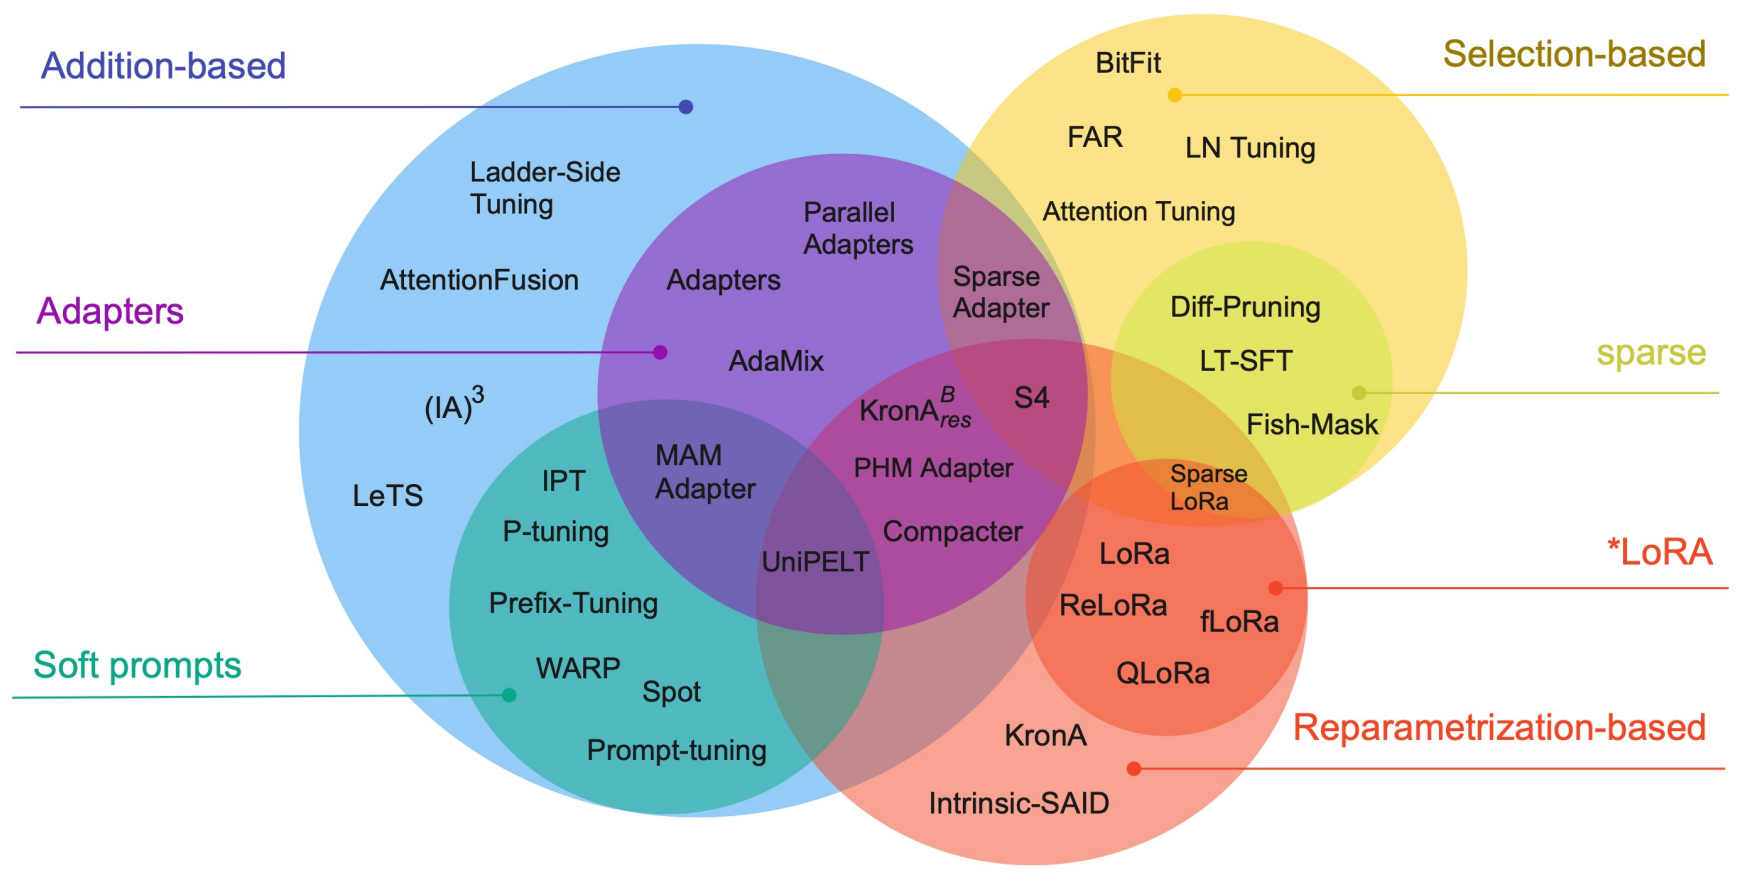
\includegraphics[width = \textwidth]{images/fine-tuning-methods-taxonomy.png}
        \caption{\footnotesize \url{https://arxiv.org/abs/2303.15647}}
      \end{figure}
    \end{column}
  \end{columns}

  
\end{frame}

\note{"Addition-based methods augment the pre-trained model with additional parameters or layers
and train only the newly introduced elements.", }

\begin{frame}{LoRA}

  \begin{itemize}
    \setlength\itemsep{1em}
    \item \textbf{Lo}w-\textbf{R}ank \textbf{A}daptation of Large Language Models
    \item \href{https://arxiv.org/abs/2106.09685}{arXiv:2106.09685}, 2021, Microsoft
    \item \url{https://github.com/microsoft/LoRA}
    \item Freezes the pretrained model weights
    \item Adding low-rank matrices into each transformer layer
  \end{itemize}

\end{frame}

\note{ }

\begin{frame}{Why LoRA?}

  \begin{itemize}
    \setlength\itemsep{1em}
    \item Minimising  memory consumption
    \item Enabling fine-tuning on hardware with limited resources
    \item Learning task-specific transformations without altering the original model structure
  \end{itemize}

\end{frame}

\note{ }


\begin{frame}{Preparing the stage}

  \begin{center}
    \Huge \color[rgb]{1,1,1}Once upon a time \dots
  \end{center}

\end{frame}

\begin{frame}{Preparing the stage}

  \begin{columns}
    \begin{column}{0.4\textwidth}
      CLI Cowboys ran the network.
    \end{column}
    \begin{column}{0.4\textwidth}
      \begin{figure}
        
\includegraphics[height = 0.7\textheight]{images/urs_cowboy.png}
        \caption{\footnotesize ChatGPT}
      \end{figure}
    \end{column}
  \end{columns}

\end{frame}

\begin{frame}{Preparing the stage}

  \begin{columns}
    \begin{column}{0.4\textwidth}
      Shooting network configs from the hips.
    \end{column}
    \begin{column}{0.4\textwidth}
      \begin{figure}
        
\includegraphics[height = 0.7\textheight]{images/urs_cli_cowboy.png}
        \caption{\footnotesize ChatGPT}
      \end{figure}
    \end{column}
  \end{columns}

\end{frame}

\begin{frame}{Preparing the stage}

  \begin{columns}
    \begin{column}{0.4\textwidth}
      Network engineers working on the neglected network dreamed about \dots
    \end{column}
    \begin{column}{0.4\textwidth}
      \begin{figure}
        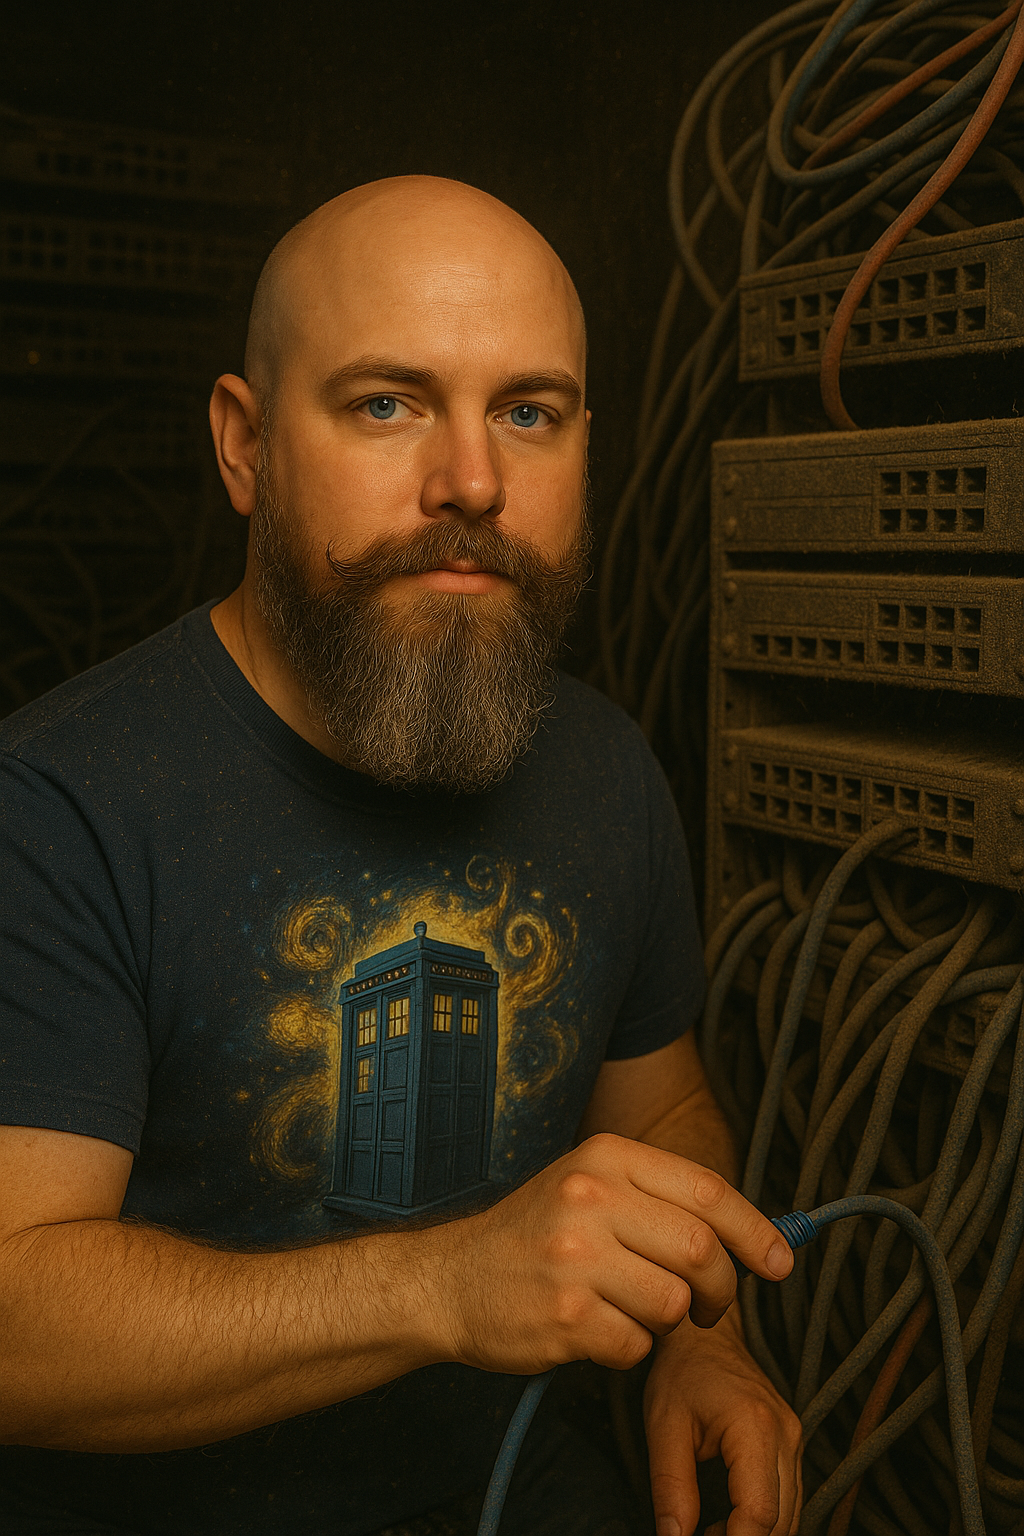
\includegraphics[height = 0.7\textheight]{images/urs_old_datacenter.png}
        \caption{\footnotesize ChatGPT}
      \end{figure}
    \end{column}
  \end{columns}

\end{frame}

\begin{frame}{Preparing the stage}

  \begin{columns}
    \begin{column}{0.4\textwidth}
      \dots a modern declarative network.
    \end{column}
    \begin{column}{0.4\textwidth}
      \begin{figure}
        
\includegraphics[height = 0.7\textheight]{images/urs_future_network.png}
        \caption{\footnotesize ChatGPT}
      \end{figure}
    \end{column}
  \end{columns}

\end{frame}

\begin{frame}{Preparing the stage}

  \begin{columns}
    \begin{column}{0.4\textwidth}
      And take time off.
    \end{column}
    \begin{column}{0.4\textwidth}
      \begin{figure}
        
\includegraphics[height = 0.7\textheight]{images/urs_hawaii.png}
        \caption{\footnotesize ChatGPT}
      \end{figure}
    \end{column}
  \end{columns}

\end{frame}

\begin{frame}{Preparing the stage}

  \begin{columns}
    \begin{column}{0.4\textwidth}
      However, they needed to extract the intent and resources from the inconsistent network configuration.
    \end{column}
    \begin{column}{0.4\textwidth}
      \begin{figure}
        
\includegraphics[height = 0.7\textheight]{images/urs_gold_rush_glory.png}
        \caption{\footnotesize ChatGPT}
      \end{figure}
    \end{column}
  \end{columns}

\end{frame}


\begin{frame}{}

  \begin{center}
    \Huge \color[rgb]{1,1,1}Intent and Resource Extraction \\ from Network Device Configuration
  \end{center}

\end{frame}


\begin{frame}{Fine-tuning Pipeline}

      \begin{figure}
        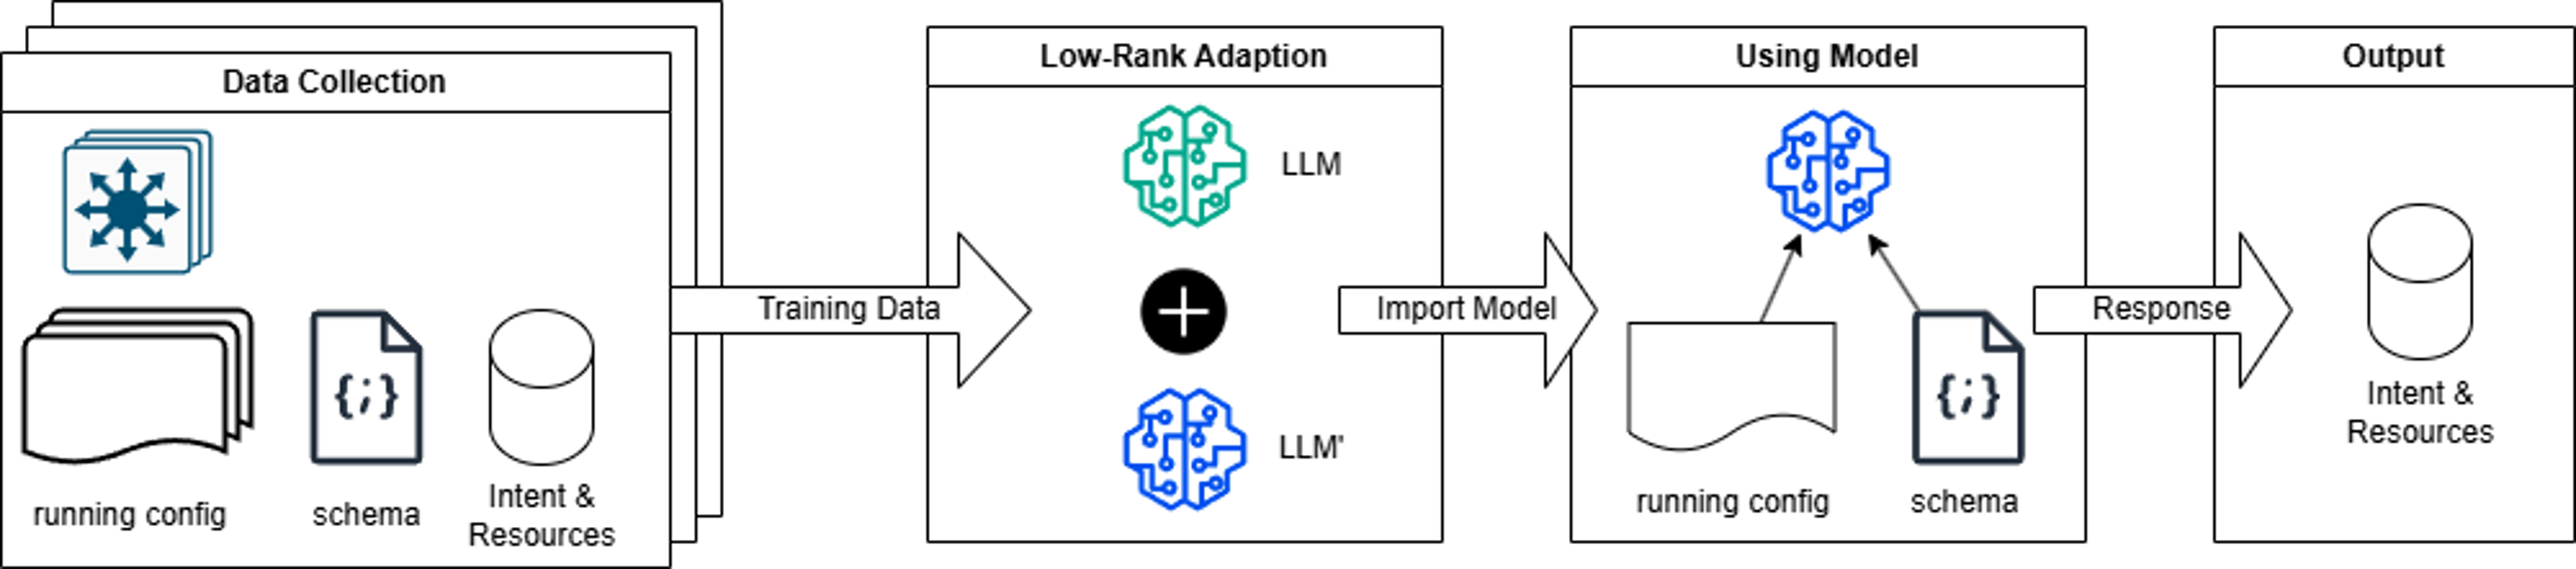
\includegraphics[width = \textwidth]{images/fine-tuning-pipeline.png}
      \end{figure}

\end{frame}

\begin{frame}{Using new model}

  \begin{figure}
    \includegraphics[width = \textwidth]{images/fine-tuning-e2e-poc.png}
  \end{figure}

\end{frame}

\begin{frame}{Evaluation}

  \texttt{Qwen2.5-Coder-32B-Instruct}

  \begin{itemize}
    \setlength\itemsep{1em}
    \item Data Extraction Match: 0.86
    \item JSON Validity: 1.0
  \end{itemize}

  \texttt{OpenAI GPT-4.0}
  \begin{itemize}
    \setlength\itemsep{1em}
    \item Data Extraction Match: 0.09
    \item JSON Validity: 0.98
  \end{itemize}

\end{frame}

\begin{frame}{Challenges}

  \begin{itemize}
    \setlength\itemsep{1em}
    \item Confusion between similar schemas
    \item IP Address + mask to CIDR
    \item Dataset quality
  \end{itemize}

\end{frame}

\begin{frame}{Lessons}

  \begin{itemize}
    \setlength\itemsep{1em}
    \item One model for each schema
    \item Generating parser template
    \item Validate dataset
    \item LLM size
  \end{itemize}

\end{frame}

\begin{frame}{Tool Stack Fine-tuning Pipeline}

  \begin{itemize}
    \setlength\itemsep{1em}
    \item \href{https://github.com/unslothai/unsloth}{unsloth}
    \item \href{https://github.com/vllm-project/vllm}{vLLM}
    \item \href{https://github.com/mlflow/mlflow}{MLflow}
  \end{itemize}

\end{frame}

\begin{frame}{Possible Improvements}

  \begin{itemize}
    \setlength\itemsep{1em}
    \item Fine-tuning for a specific schema and platform
    \item Improve training data quality
    \item Generate parser templates
    \item Hire interns
  \end{itemize}

\end{frame}


{
  \setbeamercolor{background canvas}{bg=black}
  \begin{frame}[plain,c]
    \begin{center}
      \Huge \color[rgb]{1,1,1}Thank you!
    \end{center}
  \end{frame}
}

\begin{frame}{What is missing?}

  \begin{itemize}
    \setlength\itemsep{1em}
    \item Training data sets
    \item Benchmarks
    \item Real-world showcases
  \end{itemize}

\end{frame}

\begin{frame}

  \begin{figure}
    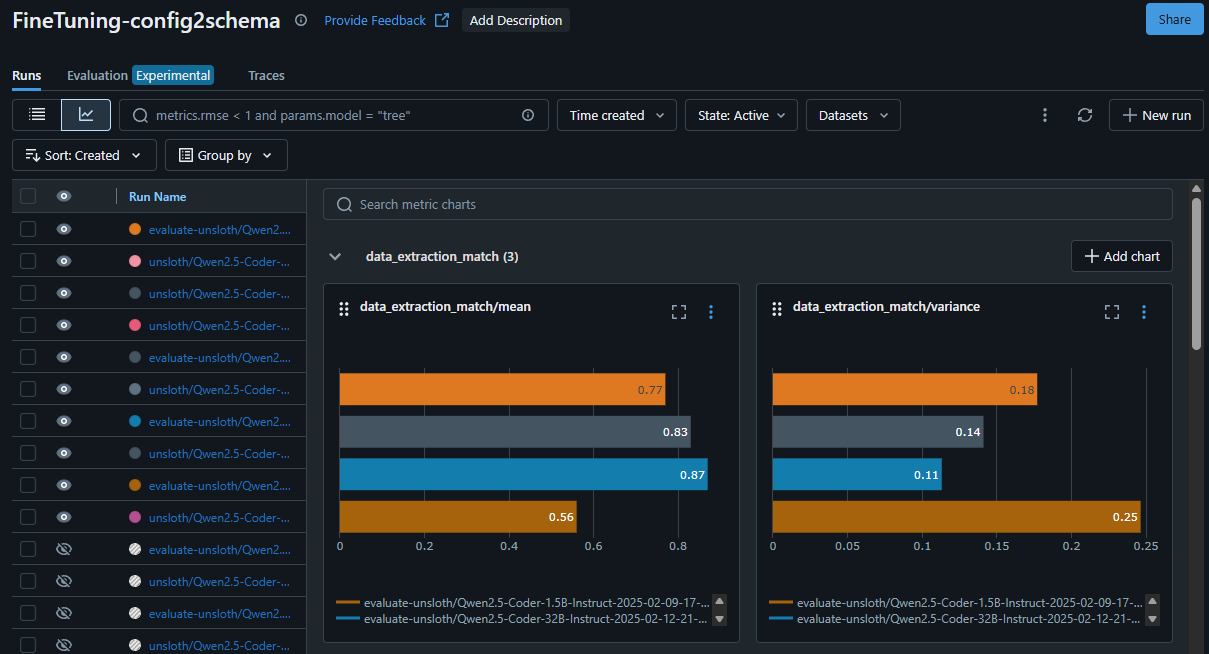
\includegraphics[width = \textwidth]{images/mlflow.png}
  \end{figure}

\end{frame}

\end{document}